\documentclass[main.tex]{subfiles}
\begin{document}

\section{Technological Background}

\subsection{Parallel Computing}

Traditional computer programs are written in a sequential manner. It is natural to think of an algorithm as a sequence of steps that can be performed serially to achieve a final result. This has actually been the most common programming paradigm since the early days of computing, and it synergizes well with single processor machines. Optimizations related to parallelism, such as out-of-order execution, branch prediction or superscalarity, were mostly handled by the compiler or the hardware itself, and transparent to the programmer. Vector processing was also a key performance factor, allowing the same instruction to be applied to a vector of data simultaneously, rather than one at a time (commonly called \ac{SIMD} instruction).

But in the beggining of the $XXI$ century, computational chips development started to shift from a single faster core perspective, to a multi core one. This was due to limitations in the evolution of single core processors, which were reaching the limits of transistor size and achievable clock frequencies, while introducing or aggravating other problems, such as heat dissipation, which becomes harder with the increased complexity of a chip. The solution was to start thinking in a multi-core perspective, coupling more cores in the same machine or even in the same die, to share the workload and allow overall computational capabilities to keep evolving.

This has allowed hardware development to keep in conformance with Moore's Law\footnote{A prediction by Gordon Moore, stating that approximately every two years, the number of transistors in a computer chip would double} \todo{ref}. And while it was a necessary step from a hardware's perspective, this has important implications in software development. In order for an application to take advantage of multi-core technology, it needs to be broken into smaller tasks, that can be executed independently, or with some level of synchronization and communication between them. Writing parallel algorithms requires an adaptation to this new paradigm, as a sequential line of execution does not provide efficient results in parallel architectures.

\subsection{Accelerators}

\begin{figure}
  \centering
  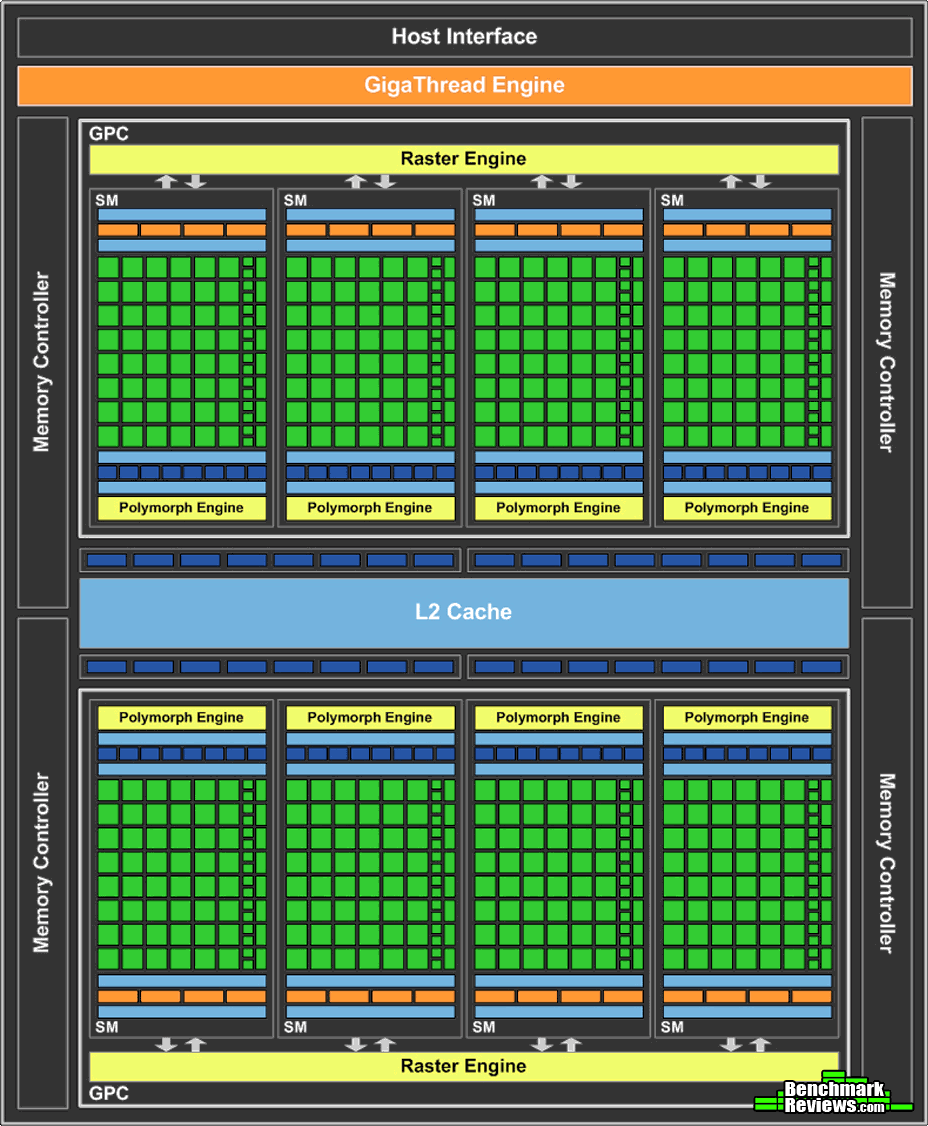
\includegraphics[width=0.6\textwidth]{arch_fermi}
  \caption{Overview of the Fermi architecture \label{fig:fermi}}
\end{figure}

\itodo{Background}

\end{document}
